\section*{\texorpdfstring{X: Decoradores: \newline  Selección de tipo dinámico}{X: Decoradores:  Selección Tipo dinámico}}
\label{sec:xdstd}
\addcontentsline{toc}{section}{\nameref{sec:xdstd}}


\textbf{El uso de objetos en capas, para añadir de forma dinámica y transparente, responsabilidades a los objetos individuales se le conoce como el patrón \textit{decorator} (decorador)}. \newline

Se utilizan cuando la subclasificación crea demasiadas (o inflexibles) clases.   \newline

Todos los decoradores que envuelven al objeto original deben tener la misma interfaz básica. \newline

Dynamic proxy/surrogate? (¿Proxy dinámico/subrogado?)  \newline

Esto explica la estructura de herencia singular.    \newline

Tradeoff:  la codificación es más complicado cuando se utiliza decoradores.

\newpage

\subsection*{Estructura Decorador básico}
\label{subsec:edb}
\addcontentsline{toc}{subsection}{\nameref{subsec:edb}}

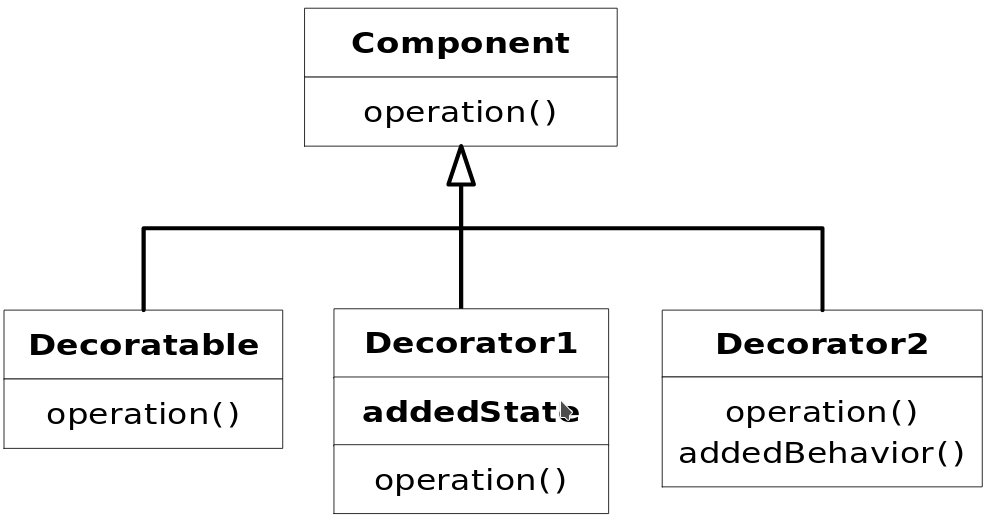
\includegraphics[width=\textwidth]{Pag73}

\subsection*{Un ejemplo café}
\label{subsec:uec}
\addcontentsline{toc}{subsection}{\nameref{subsec:uec}}

Considere la posibilidad de bajar a la cafetería local, \textit{BeanMeUp}, por un café. Normalmente hay muchas bebidas diferentes que se ofrecen \-\- expresos, cafés con leche, tés, cafés helados, chocolate caliente para nombrar unos pocos, así como una serie de extras (que cuestan extra también), tales como la crema batida o una inyección extra de expreso. Usted también puede hacer ciertos cambios en su bebida, sin costo adicional, como pedir café descafeinado en lugar de café regular.     \newline

Con bastante claridad si vamos a modelar todas estas bebidas y combinaciones, habrá diagramas de clases de tamaño variable. Así que para mayor claridad nosotros sólo consideraremos un subconjunto de los cafés: Expreso, café vienés, Caffe Latte,
Cappuccino y Café Mocha. 
Incluiremos 2 extras - crema batida ("batida") y una inyección extra de café expreso; y tres cambios - descafeinado, leche al vapor ("húmeda") y espuma de leche ("seco").   \newline

\subsection*{Clase para cada combinación}
\label{subsec:cpcc}
\addcontentsline{toc}{subsection}{\nameref{subsec:cpcc}}

Una solución es crear una clase individual  para cada combinación.Cada clase describe la bebida y es responsable por el costo, etc. El menú resultante es enorme, y una parte del diagrama de clases sería algo como esto:    \newline

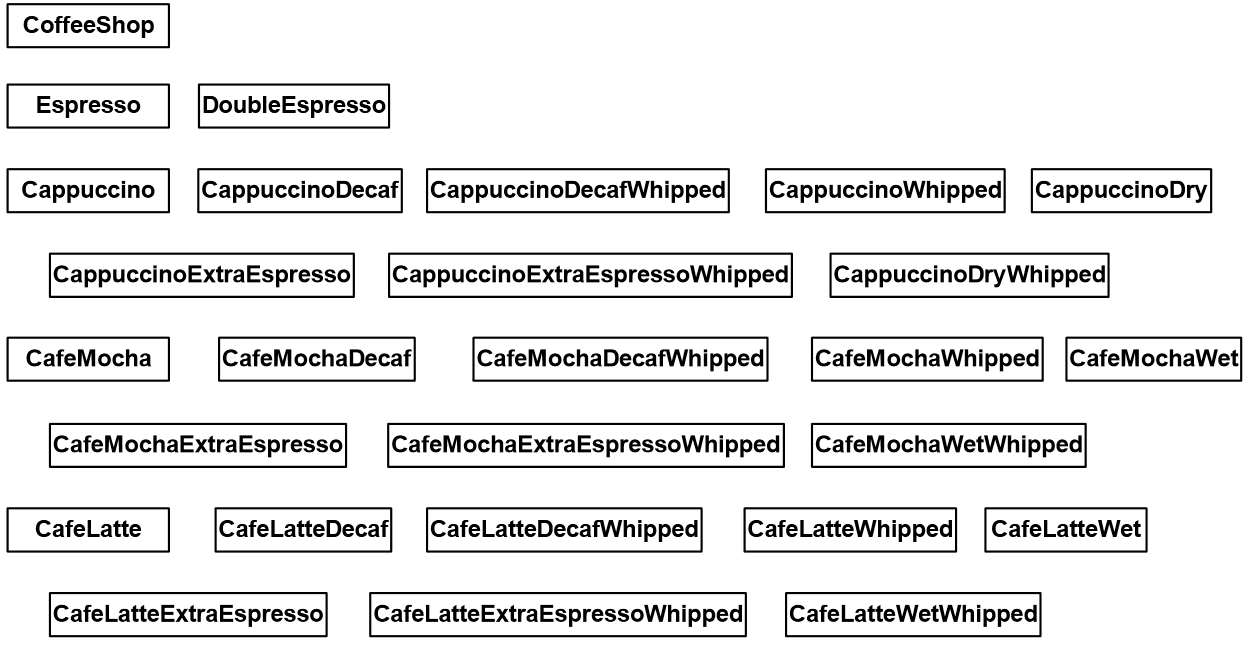
\includegraphics[width=\textwidth]{PaginaNo74} 

Aqui esta una de las combinaciones, una implementación simple de un Cappuccino:     \newline

\begin{lstlisting} 
class Cappuccino: 
  def __init__(self): 
    self.cost = 1 
    self.description = "Cappucino" 
  def getCost(self): 
    return self.cost 
  def getDescription(self): 
    return self.description 
\end{lstlisting}

La clave para el uso de este método es encontrar la combinación particular que desea. Así, una vez que haya encontrado la bebida que le gustaría, aquí le presentamos una forma de hacerlo, como se muestra en la clase \textbf{CoffeeShop} en el siguiente código:     \newline

\begin{lstlisting}
#: cX:decorator:nodecorators:CoffeeShop.py 
# Coffee example with no decorators 

class Espresso: pass 
class DoubleEspresso: pass

class EspressoConPanna: pass 

class Cappuccino: 
  def __init__(self): 
    self.cost = 1 
    self.description = "Cappucino" 
  def getCost(self): 
    return self.cost 
  def getDescription(self): 
    return self.description 
    
class CappuccinoDecaf: pass 
class CappuccinoDecafWhipped: pass 
class CappuccinoDry: pass 
class CappuccinoDryWhipped: pass 
class CappuccinoExtraEspresso: pass 
class CappuccinoExtraEspressoWhipped: pass 
class CappuccinoWhipped: pass 

class CafeMocha: pass 
class CafeMochaDecaf: pass 
class CafeMochaDecafWhipped: 
  def __init__(self): 
    self.cost = 1.25 
    self.description = \ 
      "Cafe Mocha decaf whipped cream" 
  def getCost(self): 
    return self.cost 
  def getDescription(self): 
    return self.description 
    
class CafeMochaExtraEspresso: pass 
class CafeMochaExtraEspressoWhipped: pass 
class CafeMochaWet: pass 
class CafeMochaWetWhipped: pass 
class CafeMochaWhipped: pass 

class CafeLatte: pass 
class CafeLatteDecaf: pass 
class CafeLatteDecafWhipped: pass 
class CafeLatteExtraEspresso: pass 
class CafeLatteExtraEspressoWhipped: pass 
class CafeLatteWet: pass 
class CafeLatteWetWhipped: pass 

class CafeLatteWhipped: pass 
cappuccino = Cappuccino() 
print (cappuccino.getDescription() + ": \$" +  
  `cappuccino.getCost()`) 
  
cafeMocha = CafeMochaDecafWhipped() 
print (cafeMocha.getDescription() 
  + ": \$" + `cafeMocha.getCost()`) 
#:~ 
\end{lstlisting}

y aquí está la salida correspondiente: \newline

\begin{lstlisting} 
Cappucino: $1.0Cafe Mocha decaf whipped cream: $1.25
\end{lstlisting}

Se puede ver que la creación de la combinación particular que se desea es fácil, ya que sólo está creando una instancia de una clase. Sin embargo, hay una serie de problemas con este enfoque. En primer lugar, las combinaciones son fijadas estáticamente para que cualquier combinación de un cliente que, quizá desee ordenar, necesite ser creada por adelantado. En segundo lugar, el menú resultante es tan grande que la búsqueda de su combinación particular es difícil y consume mucho tiempo.     \newline


\subsection*{El enfoque decorador}
\label{subsec:eed}
\addcontentsline{toc}{subsection}{\nameref{subsec:eed}}

Otro enfoque sería descomponer las bebidas en los diversos componentes, tales como expreso y leche espumada, y luego dejar que el cliente combine los componentes para describir un café en particular.    \newline

Con el fin de hacer esto mediante programación, utilizamos el patrón Decorador. Un decorador añade la responsabilidad de un componente envolviéndolo, pero el decorador se ajusta a la interfaz del componente que encierra, por lo que la envoltura es transparente. Los Decoradores también se pueden anidar sin la pérdida de esta transparencia. \newline

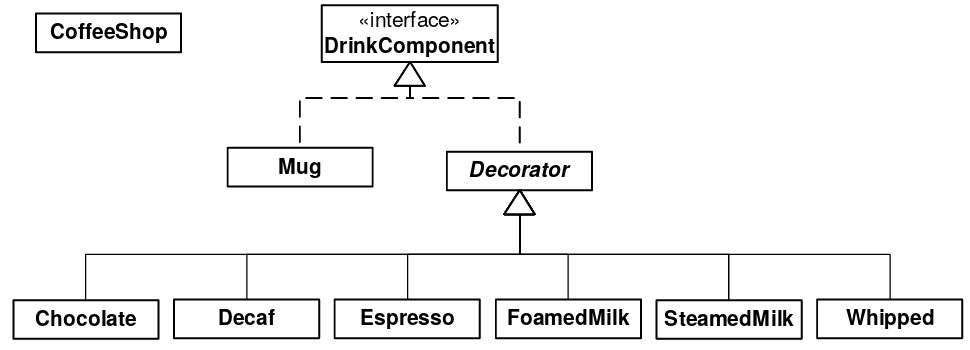
\includegraphics[width=\textwidth]{Pag77}

Métodos invocados en el Decorador a su vez pueden invocar métodos en el componente, y puede realizar, por supuesto, el procesamiento antes o después de la invocación.   \newline

Así que si añadimos los métodos \textbf{getTotalCost()} y \textbf{getDescription()} a la interfaz \textbf{DrinkComponent}, un Espresso se ve así:     \newline

\begin{lstlisting} 
class Espresso(Decorator): 
  cost = 0.75f 
  description = " espresso" 
  public Espresso(DrinkComponent): 
    Decorator.__init__(self, component) 
    
  def getTotalCost(self): 
    return self.component.getTotalCost() + cost 
    
  def getDescription(self): 
    return self.component.getDescription() + 
      description 
\end{lstlisting}

Usted combina los componentes para crear una bebida de la siguiente manera, como se muestra en el siguiente código:     \newline

\begin{lstlisting} 
#: cX:decorator:alldecorators:CoffeeShop.py 
# Coffee example using decorators

class DrinkComponent: 
  def getDescription(self): 
    return self.__class__.__name__ 
  def getTotalCost(self): 
    return self.__class__.cost 
    
class Mug(DrinkComponent): 
  cost = 0.0 
  
class Decorator(DrinkComponent): 
  def __init__(self, drinkComponent): 
    self.component = drinkComponent 
  def getTotalCost(self): 
    return self.component.getTotalCost() + \ 
      DrinkComponent.getTotalCost(self) 
  def getDescription(self): 
    return self.component.getDescription() + \ 
      ' ' + DrinkComponent.getDescription(self) 
      
class Espresso(Decorator): 
  cost = 0.75 
  def __init__(self, drinkComponent): 
    Decorator.__init__(self, drinkComponent) 
    
class Decaf(Decorator): 
  cost = 0.0 
  def __init__(self, drinkComponent): 
    Decorator.__init__(self, drinkComponent) 
    
class FoamedMilk(Decorator): 
  cost = 0.25 
  def __init__(self, drinkComponent): 
    Decorator.__init__(self, drinkComponent) 
    
class SteamedMilk(Decorator): 
  cost = 0.25 
    def __init__(self, drinkComponent): 
    Decorator.__init__(self, drinkComponent) 
class Whipped(Decorator): 
  cost = 0.25 
  def __init__(self, drinkComponent): 
    Decorator.__init__(self, drinkComponent) 
class Chocolate(Decorator): 
  cost = 0.25 
  def __init__(self, drinkComponent): 
    Decorator.__init__(self, drinkComponent) 
cappuccino = Espresso(FoamedMilk(Mug())) 
print cappuccino.getDescription().strip() + \ 
  ": \$" + `cappuccino.getTotalCost()`
  
cafeMocha = Espresso(SteamedMilk(Chocolate( 
  Whipped(Decaf(Mug()))))) 
  
print cafeMocha.getDescription().strip() + \ 
  ": \$" + `cafeMocha.getTotalCost()` 
#:~ 
\end{lstlisting}

Este enfoque, sin duda, proporciona la mayor flexibilidad y el menú más pequeño. Usted tiene un pequeño número de componentes para elegir,  pero el montaje de la descripción del café entonces se vuelve bastante arduo.   \newline

Si quiere describir un capuchino sencillo, se crea con \newline

\begin{lstlisting} 
plainCap = Espresso(FoamedMilk(Mug()))
\end{lstlisting}

Creando un Café Mocha descafeinado con crema batida requiere una descripción aún más larga. \newline


\subsection*{Compromiso}
\label{subsec:c}
\addcontentsline{toc}{subsection}{\nameref{subsec:c}}

El enfoque anterior toma demasiado tiempo para describir un café. También habrá ciertas combinaciones que se irán describiendo de manera regular, y sería conveniente tener una forma rápida de describirlos.     \newline

El tercer enfoque es una mezcla de los 2 primeros enfoques, y combina flexibilidad con la facilidad de uso. Este compromiso se logra mediante la creación de un menú de tamaño razonable de opciones básicas, que a menudo funcionan exactamente como son, pero si quería decorarlos (crema batida, descafeinado etc), entonces usted usaría decoradores para hacer las modificaciones. Este es el tipo de menú que se le presenta en la mayoría de tiendas de café.    \newline

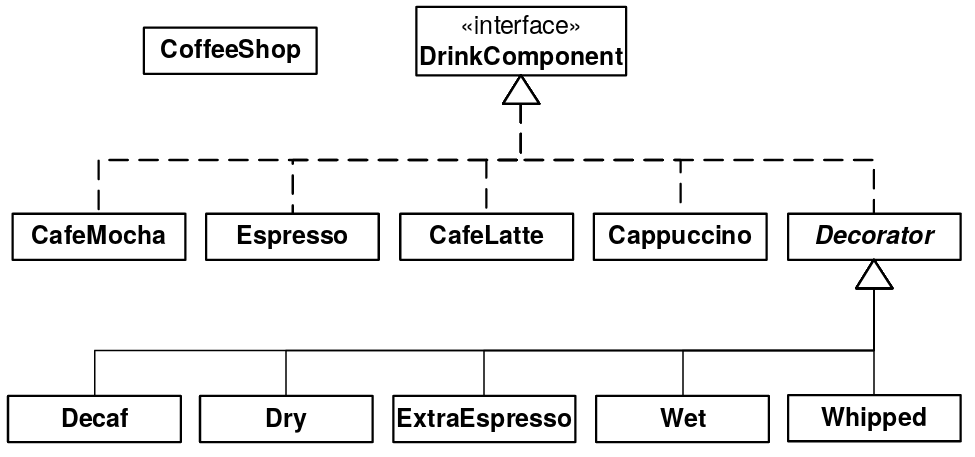
\includegraphics[width=\textwidth]{Pag80}

Se muestra cómo crear una selección básica, así como una selección decorada:     \newline

\begin{lstlisting} 
#: cX:decorator:compromise:CoffeeShop.py 
# Coffee example with a compromise of basic 
# combinations and decorators 

class DrinkComponent: 
  def getDescription(self): 
    return self.__class__.__name__ 
  def getTotalCost(self): 
    return self.__class__.cost 
    
class Espresso(DrinkComponent): 
  cost = 0.75 
  
class EspressoConPanna(DrinkComponent): 
  cost = 1.0 
  
class Cappuccino(DrinkComponent): 
  cost = 1.0 
  
class CafeLatte(DrinkComponent): 
  cost = 1.0 
  
class CafeMocha(DrinkComponent): 
  cost = 1.25 
  
class Decorator(DrinkComponent): 
  def __init__(self, drinkComponent): 
    self.component = drinkComponent 
  def getTotalCost(self): 
      return self.component.getTotalCost() + \ 
      DrinkComponent.getTotalCost(self) 
  def getDescription(self): 
    return self.component.getDescription() + \ 
      ' ' + DrinkComponent.getDescription(self) 
      
class ExtraEspresso(Decorator): 
  cost = 0.75 
  def __init__(self, drinkComponent): 
    Decorator.__init__(self, drinkComponent) 
    
class Whipped(Decorator): 
  cost = 0.50 
  def __init__(self, drinkComponent): 
    Decorator.__init__(self, drinkComponent) 
    
class Decaf(Decorator): 
  cost = 0.0 
  def __init__(self, drinkComponent): 
    Decorator.__init__(self, drinkComponent) 
    
class Dry(Decorator): 
      cost = 0.0 
  def __init__(self, drinkComponent): 
    Decorator.__init__(self, drinkComponent) 
    
class Wet(Decorator): 
  cost = 0.0 
  def __init__(self, drinkComponent): 
    Decorator.__init__(self, drinkComponent) 
    
cappuccino = Cappuccino() 
print cappuccino.getDescription() + ": \$" + \ 
  `cappuccino.getTotalCost()` 
  
cafeMocha = Whipped(Decaf(CafeMocha())) 
print cafeMocha.getDescription() + ": \$" + \ 
  `cafeMocha.getTotalCost()` 
#:~ 
\end{lstlisting}

Usted puede ver que creando una selección básica es rápido y fácil, lo cual tiene sentido ya que serán descritos con regularidad. Describiendo una bebida decorada hay más trabajo que cuando se utiliza una clase por combinación, pero claramente menos trabajo que cuando se usan solo los decoradores.    \newline

El resultado final no es demasiadas clases, ni tampoco demasiados decoradores. La mayoría de las veces es posible alejarse sin utilizar ningún decorador en absoluto, así tenemos los beneficios de ambos enfoques.     \newline


\subsection*{Otras consideraciones}
\label{subsec:oc}
\addcontentsline{toc}{subsection}{\nameref{subsec:oc}}


¿Qué sucede si decidimos cambiar el menú en una etapa posterior, tal como mediante la adición de un nuevo tipo de bebida? Si hubiéramos utilizado la clase por enfoque de combinación, el efecto de la adición de un ejemplo adicional como Syrup sería un crecimiento exponencial en el número de clases. Sin embargo, las implicaciones para todos los enfoques decorador o de compromiso son los mismos \- , se crea una clase extra.    \newline

¿Qué tal el efecto de cambiar el costo de la leche al vapor y espuma de leche, cuando el precio de la leche sube? Teniendo una clase para cada combinación significa que usted necesita cambiar un método en cada clase, y así mantener muchas clases. Mediante el uso de decoradores, el mantenimiento se reduce mediante la definición de la lógica en un solo lugar.  \newline

\subsection*{Ejercicios}
\label{subsec:ejer}
\addcontentsline{toc}{subsection}{\nameref{subsec:ejer}}

\begin{enumerate}[1.]
    \item Añadir una clase Syrup al enfoque decorador descrito anteriormente. A continuación, cree un Café Latte (usted necesitará usar la leche al vapor con un expreso) con Syrup.
    \item Repita el ejercicio 1 para el enfoque de compromiso.
    \item Implementar el patrón decorador para crear un restaurante de Pizza, el cual tenga un menú de opciones, así como la opción de diseñar su propia pizza. Siga el enfoque de compromiso para crear un menú que consiste en una margherita, hawaianas, regina, y pizzas vegetarianas, con relleno (decoradores) de ajo, aceitunas, espinacas, aguacate, queso feta y Pepperdews. Crear una pizza hawaiana, así como un Margherita decorado con espinacas, queso feta, Pepperdews y aceitunas.
\end{enumerate}

\newpage
